\documentclass{urdpl}     % praca w języku polskim

% Lista wszystkich języków stanowiących języki pozycji bibliograficznych użytych w pracy.
% (Zgodnie z zasadami tworzenia bibliografii każda pozycja powinna zostać utworzona zgodnie z zasadami języka, w którym dana publikacja została napisana.)
\usepackage[english,polish]{babel}

% Użyj polskiego łamania wyrazów (zamiast domyślnego angielskiego).
\usepackage{polski}

\usepackage[utf8]{inputenc}

% dodatkowe pakiety

\usepackage{mathtools}
\usepackage{amsfonts}
\usepackage{amsmath}
\usepackage{amsthm}
\usepackage[hidelinks]{hyperref}
\usepackage{float}
\usepackage{listings}
\usepackage{graphicx}
\usepackage{subcaption}
\usepackage{booktabs} % Dla \toprule, \midrule, \bottomrule
\usepackage{multirow} 
\usepackage{tabularx} 
\usepackage{amssymb} 
\usepackage{listings}
\usepackage{xcolor}
\usepackage{array}
\usepackage{makecell}
\usepackage[flushleft]{threeparttable}
\usepackage[normalem]{ulem}
\usepackage{lineno}
\usepackage{makecell} %
\usepackage{csquotes}
\usepackage{courier}

% ------------------------
% --- < listingi > ---

\usepackage{listings}
\lstloadlanguages{TeX}
\renewcommand{\lstlistlistingname}{Spis listingów}
\renewcommand{\lstlistingname}{Listing}

\lstset{
	literate={ą}{{\k{a}}}1
           {ć}{{\'c}}1
           {ę}{{\k{e}}}1
           {ó}{{\'o}}1
           {ń}{{\'n}}1
           {ł}{{\l{}}}1
           {ś}{{\'s}}1
           {ź}{{\'z}}1
           {ż}{{\.z}}1
           {Ą}{{\k{A}}}1
           {Ć}{{\'C}}1
           {Ę}{{\k{E}}}1
           {Ó}{{\'O}}1
           {Ń}{{\'N}}1
           {Ł}{{\L{}}}1
           {Ś}{{\'S}}1
           {Ź}{{\'Z}}1
           {Ż}{{\.Z}}1,
	basicstyle=\footnotesize\ttfamily,
}

% defninicja stylu python
\lstdefinestyle{stylePython}{
    language=Python,
    commentstyle=\color{green},          % Kolor komentarzy
    keywordstyle=\color{blue},           % Kolor słów kluczowych
    numberstyle=\tiny\color{gray},       % Kolor i styl numerów linii
    stringstyle=\color{red},             % Kolor ciągów znaków
    basicstyle=\ttfamily\footnotesize,   % Podstawowy styl kodu
    breakatwhitespace=false,             % Automatyczne dzielenie wierszy
    breaklines=true,                     % Dzielenie długich linii
    keepspaces=true,                     % Zachowanie spacji
    numbers=left,                        % Numery linii po lewej
    numbersep=5pt,                       % Odstęp numerów od kodu
    showspaces=false,                    % Nie pokazuj spacji
    showstringspaces=false,              % Nie pokazuj spacji w ciągach znaków
    showtabs=false,                      % Nie pokazuj tabulacji
    tabsize=2                            % Rozmiar tabulacji
}

% defnicja stylu JAVA
\lstdefinestyle{javaStyle}{
    language=Java,
    basicstyle=\ttfamily\footnotesize,
    keywordstyle=\color{blue},
    commentstyle=\color{green!50!black}\itshape,
    stringstyle=\color{green},
    numberstyle=\tiny\color{gray},
    numbers=left,
    numbersep=5pt,                       % Odstęp numerów od kodu
    stepnumber=1,
    showspaces=false,                    % Nie pokazuj spacji
    tabsize=2,
    showstringspaces=false,
    breaklines=true,
    breakatwhitespace=false,             % Automatyczne dzielenie wierszy
    showtabs=false,                      % Nie pokazuj tabulacji
    keepspaces=true                    % Zachowanie spacji
}

\definecolor{stringcolor}{RGB}{163,21,21}    % pomarańczowy - stringi
\definecolor{typecolor}{RGB}{43, 145, 176}     % ciemny fiolet - klasy, typy

\lstdefinestyle{csStyle}{
    language=[Sharp]C, % dla C#; można zmienić na Java
    basicstyle=\ttfamily\footnotesize,
    keywordstyle=\color{blue},
    stringstyle=\color{stringcolor},
    commentstyle=\color{green!50!black}\itshape,
    morekeywords={class, public, private, protected, static, void, string, int, new}, % dodatkowe słowa kluczowe
    emphstyle=\color{typecolor}\bfseries, % klasy na fioletowo
    numbers=left,
    numbersep=5pt,                       % Odstęp numerów od kodu
    numberstyle=\tiny\color{gray},
    stepnumber=1,
    breaklines=true,
    showspaces=false,                    % Nie pokazuj spacji
    tabsize=2,
    showstringspaces=false,
    breakatwhitespace=false,             % Automatyczne dzielenie wierszy
    showtabs=false,                      % Nie pokazuj tabulacji
    keepspaces=true                    % Zachowanie spacji  
}

\lstdefinestyle{matlabStyle}{
    language=Matlab,
    basicstyle=\ttfamily\footnotesize,  % Mała czcionka monospaced
    keywordstyle=\color{blue}\bfseries, % Słowa kluczowe na niebiesko i pogrubione
    stringstyle=\color{red},            % Ciągi znaków na czerwono
    commentstyle=\color{green!50!black}\itshape, % Komentarze na zielono, kursywa
    morekeywords={figure, imread, imshow, title, imhist, histeq, graythresh, imbinarize, stretchlim, imadjust}, % Dodatkowe słowa kluczowe MATLAB
    numbers=left,                        % Numeracja linii po lewej
    numbersep=5pt,                       % Odstęp numerów od kodu
    numberstyle=\tiny\color{gray},       % Mała, szara czcionka numerów linii
    stepnumber=1,                         % Numeracja co 1 linię
    breaklines=true,                      % Łamanie długich linii
    showspaces=false,                     % Nie pokazuj spacji
    showstringspaces=false,               % Nie pokazuj spacji w stringach
    showtabs=false,                        % Nie pokazuj tabulatorów
    tabsize=4,                             % Tabulacja 4 spacje
    breakatwhitespace=false,               % Automatyczne łamanie wierszy
    keepspaces=true                        % Zachowanie spacji  
}

\definecolor{lightgray}{rgb}{0.9,0.9,0.9}
    % \definecolor{blue}{rgb}{0,0,1}
    \definecolor{green}{rgb}{0,0.6,0}
    % \definecolor{red}{rgb}{0.6,0,0}
    \definecolor{gray}{rgb}{0.5,0.5,0.5}

% % ------------------------
\AtBeginDocument{
	\renewcommand{\tablename}{Tabela}
	\renewcommand{\figurename}{Rys.}   
    \newcommand{\listingname}{Listing}
}

% ------------------------
% --- < tabele > ---

% defines the X column to use m (\parbox[c]) instead of p (`parbox[t]`)
\newcolumntype{C}[1]{>{\hsize=#1\hsize\centering\arraybackslash}X}


%---------------------------------------------------------------------------

\author{Julia Chmura, Dominik Dziadosz}
\shortauthor{J.cChmura, D. Dziadosz}
\noAlbum{jc131414, dd131428}

\titlePL{Projekt zaliczeniowy - "Weryfikacja głosowa na stronie internetowej"}
\titleEN{Thesis in \LaTeX}

\shorttitlePL{Laboratorium z Biometrycznych Systemów Zabezpieczeń} % skrócona wersja tytułu jeśli jest bardzo długi
\shorttitleEN{Preparation of a long and fascinating thesis in \LaTeX}

\thesistype{Projekt \\ Grupa: 02}

\thesisDone{Prowadzący}
\supervisor{dr Zbigniew Gomółka}
%\supervisor{Jan Nowak PhD}

\degreeprogramme{Informatyka}
%\degreeprogramme{Computer Science}

\date{2025}

\department{Instytut Informatyki}
%\department{Institute of Computer Science}

\faculty{Wydział Nauk Ścisłych i Technicznych}
%\faculty{Faculty of Science and Technology}



\setlength{\cftsecnumwidth}{10mm}

%---------------------------------------------------------------------------
\setcounter{secnumdepth}{4}
\brokenpenalty=10000\relax

% --------------------------------------------------------------------------
% główna część pracy
% --------------------------------------------------------------------------

\begin{document}

\titlepages

% Ponowne zdefiniowanie stylu `plain`, aby usunąć numer strony z pierwszej strony spisu treści i poszczególnych rozdziałów.
\fancypagestyle{plain}
{
    % Usuń nagłówek i stopkę
    \fancyhf{}
    % Usuń linie.
    \renewcommand{\headrulewidth}{0pt}
    \renewcommand{\footrulewidth}{0pt}
}

\setcounter{tocdepth}{2}
\tableofcontents
\clearpage

% dodanie poszczególnych rozdziałów 
\chapter{Informacje ogólne}
\label{cha:Lab001}
\makeatletter


% *********************************************************************
% w poniższej metryczce należy uzupełnić informacje o:
% - temacie ćwiczenia
% - numer ćwiczenia
% - numer grupy laboratoryjnej
% - numer zespołu
% - datę wykonania ćwiczenia oraz oddania ćwiczenia.
% *********************************************************************

\begin{table}[H]
    \centering
    \renewcommand{\tabularxcolumn}[1]{m{#1}}  % Dostosowanie kolumny do zawartości
    \newcolumntype{C}{>{\centering\arraybackslash}X}
    \begin{tabularx}{\linewidth}{|C|C|}
        \hline
        \multicolumn{2}{|c|}{\makecell{\textbf{\Large{Biometryczne Systemy Zabezpieczeń}} \\ \textbf{Projekt}}} \\ \hline
        \multicolumn{1}{|l|}{Temat}                    &           Weryfikacja głosowa na stronie internetowej                \\ \hline
        \multicolumn{1}{|l|}{Technologie}                       &       Python, framework - Flask, platforma FFmpeg               \\ \hline
        \multicolumn{1}{|l|}{Biometryka}                    &           Voice             \\ \hline
        \multicolumn{1}{|l|}{Autorzy}                         &   \@author                              \\ \hline
        \multicolumn{1}{|l|}{Grupa laboratoryjna}                       &       02               \\ \hline
        
        
    \end{tabularx}
\end{table}


\section{Opis ogólny projektu}
Celem projektu jest przedstawienie komponentu biometrycznego - voice. Głos człowieka może być zastosowany jako unikalne zabezpieczenie (np. podczas logowania, lub innego zabezpieczenia zasobów). Komponent ten został zaimplementowany na stronie internetowej jako zabezpieczenie konta użytkownika. Użytkownik ma możliwość nagrać próbkę swojego głosu z wypowiadając daną frazę, a następnie przechodząc do logowania nagrywa ponownie próbkę głosu z tą samą frazą, po czym następuje weryfikacja. Obsługa komponentu biometrycznego została napisana w pythonie z użyciem odpowiednich bibliotek, a prosta witryna internetowa do jego wykorzystania została napisana we frameworku pythona - Flask. 

\section{Wstęp teoretyczny}



\section{Opis wykorzystywanego oprogramowania i narzędzi}
\begin{itemize}
	\item \textbf{Python} - główny język programowania na którym opiera się cały projekt
	\item \textbf{Flask} - framework Pythona który posłużył do stworzenia szaty graficznej projektu (strony internetowej na której odbywa się weryfikacja głosowa)
	\item Biblioteki Pythona
	\begin{itemize}
		\item \textbf{numpy} - jest jedną z głównych elementów projektu. Wykorzystana została do stworzenia tablicy jednowymiarowej w której przechowywane są liczby zmiennoprzecinkowe stworzone przez inną bibliotekę librosa, reprezentujące głos. Potrzebna jest również do uproszczenia operacji matematycznych oraz pozwala na zarządzanie macierzami zawartymi w kodzie
		\item \textbf{librosa} - biblioteka ta w projekcie ma szczególnie zadanie, odpowiada ona za cały aspekt analizy dźwięku. Dzięki niej wczytywany jest głos oraz dekodowany, wstępnie oczyszcza dźwięk (np. usuwa sekundy ciszy z nagrania) oraz najważniejsze odpowiada za wydobycie cech biometrycznych z głosu.
		\item \textbf{SciPy  moduł scipy.spatial.distance} - biblioteka ta to olbrzymi zbiór gotowych maszyn i narzędzi matematycznych, inżynierskich i naukowych
		\item \textbf{pydub} - ta biblioteka posłużyła jako narzędzie do manipulacji i przetwarzania plików audio. W kontekście projektu jej główna rola to przyjmowanie plików głosowych, a następnie konwertuje je do formatu WAV. 
		\item \textbf{os} - biblioteka ta posłużyła do obsługi plików i folderów
		
	\end{itemize}	
\end{itemize}	



\section{Działanie programu}
Działanie projektu zaczynamy od strony głównej na której jest rejestracja i logowanie. W pierwszym kroku użytkownik rejestruje się nagrywając próbkę głosu. 

\begin{figure}[H]
	\centering
	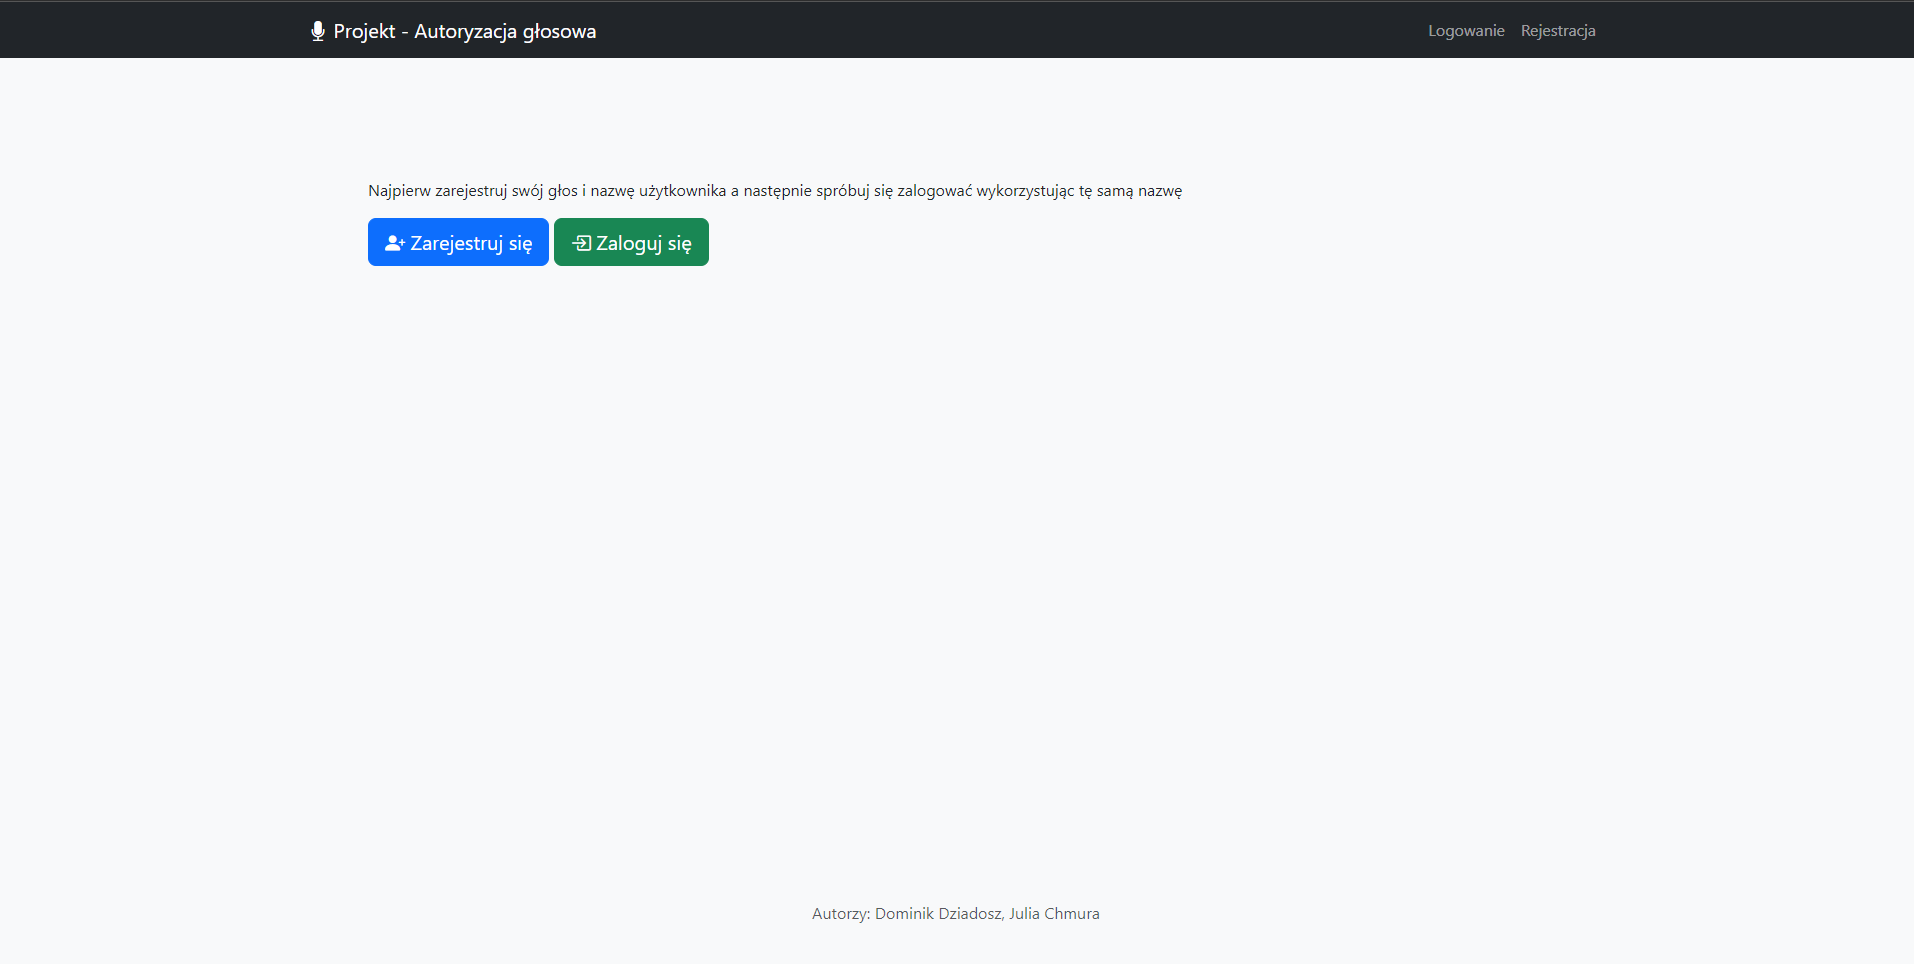
\includegraphics[width=\linewidth]{src/images/strona_glowna.png}
	\caption{Obraz strony głównej}
\end{figure}

Po kliknięciu "Zarejestruj się" przechodzimy do strony rejestracji. Tutaj podawana jest nazwa użytkownika i nagrywana próbka głosu (około 2 do 3 sekundy). 

\begin{figure}[H]
	\centering
	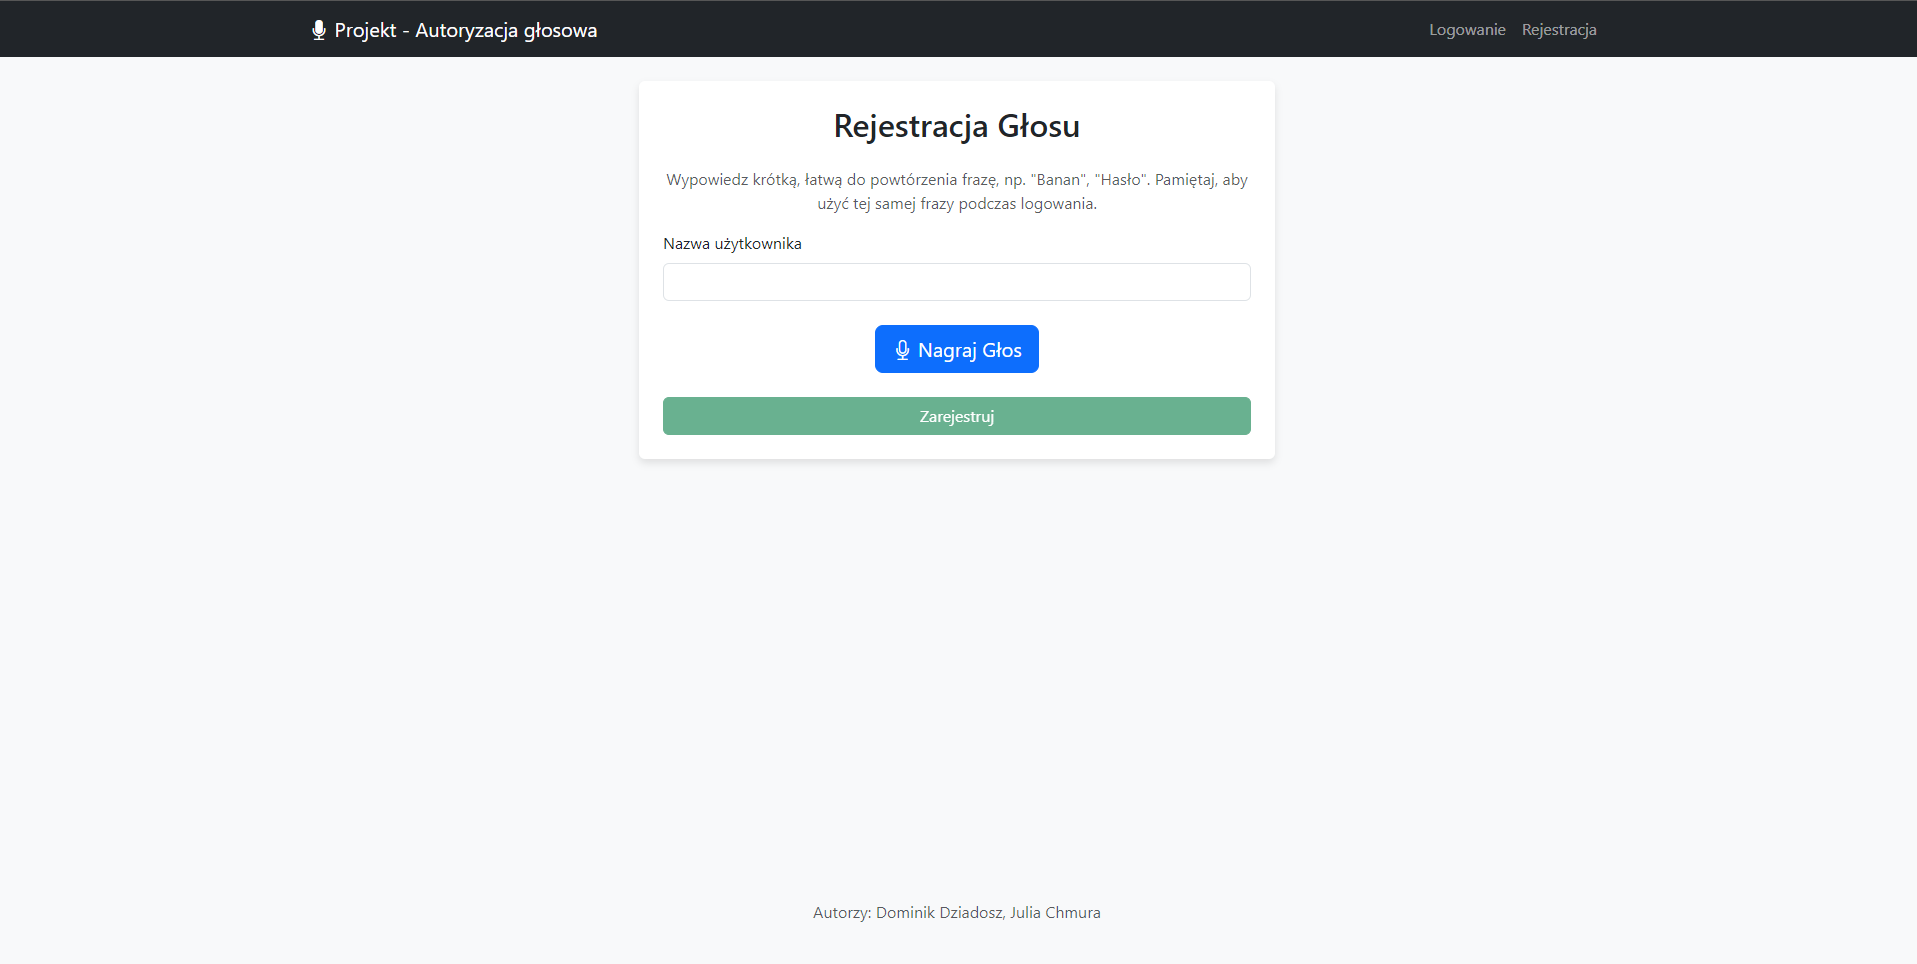
\includegraphics[width=\linewidth]{src/images/nagranie_probki_glosu.png}
	\caption{Obraz strony rejestracji}
\end{figure}

Po zarejestrowaniu się należy przejść do logowania. Tutaj ponownie podajemy nazwę użytkownika i nagrywana jest kolejna próbka, która jest porównywana do tej podanej podczas rejestracji. Jeżeli próbki będą zgodne, użytkownik przechodzi poprawnie przez weryfikację lub nie przechodzi, w każdym przypadku zostaje o tym poinformowany stosownym komunikatem. 

\begin{figure}[H]
	\centering
	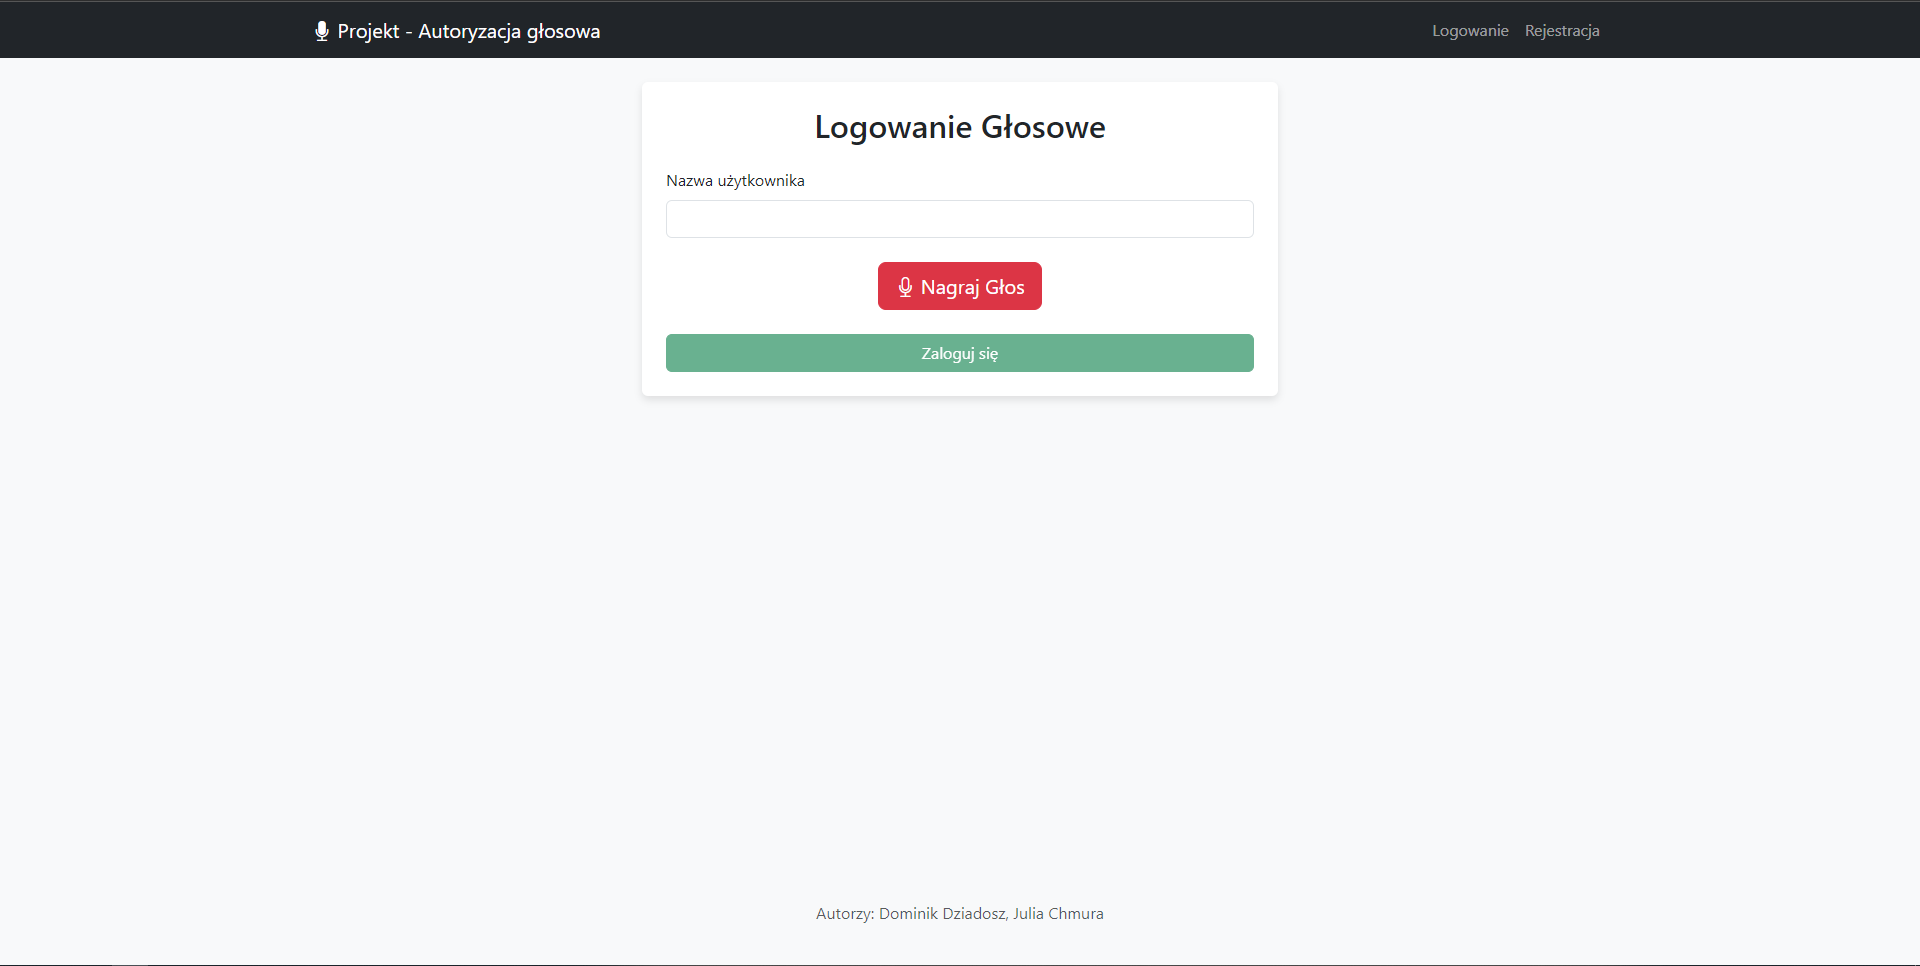
\includegraphics[width=\linewidth]{src/images/weryfikacja_probki_glosu.png}
	\caption{Obraz strony logowania}
\end{figure}

\section{Instrukcja nagrywania próbki głosu}
Aby poprawnie nagrać próbkę głosu należy spełnić dane warunki:
\begin{itemize}
	\item Przygotować odpowiedni sprzęt: poprawnie działający mikrofon
	\item Mówić jednolitym tonem 
	\item Wypowiedzieć proste hasło, najlepiej zkładające się z dwóch słów
	\item Przy rejestracji i logowaniu posłużyć się tym samym zwrotem, mówiąc w takim samym tonie i tempie
	\item Upewnić się że nagrania nie zakłucają odgłosy z otoczenia
	\item Nagrać próbkę trwającą około dwie lub trzy sekundy
	
\end{itemize}


\section{Wnioski}
Na podstawie przeprowadzonych eksperymentów można stwierdzić, że:
\begin{itemize}
    \item Histogram jest przydatnym narzędziem w analizie jakości obrazu biometrycznego.
    \item Wyrównanie histogramu poprawia kontrast i może zwiększać czytelność obrazu.
    \item Segmentacja oparta na histogramie, w szczególności metoda Otsu, pozwala na skuteczne wydzielenie istotnych cech obrazu.
\end{itemize}

\section{Bibliografia}
\begin{itemize}
    \item MATLAB Image Processing Toolbox Documentation \cite{mathworks},
    \item Rafael Gonzalez, Richard Woods, Digital Image Processing Global Edition \cite{gonzalez2017}.
    \item Flask Documentation. Pallets.  \cite{flask_docs}
    \item Pydub Documentation. Read the Docs.  \cite{pydub_docs}
    \item Librosa Documentation  \cite{librosa_docs}
    \item SciPy Documentation  \cite{scipy_docs}
    \item NumPy Documentation \cite{numpy_docs}
    \item scikit-learn Documentation  \cite{scikitlearn_docs}
    \item FFmpeg Documentation  \cite{ffmpeg_docs}
    
\end{itemize}


% Wyłączenie działania `ulem` na czas bibliografii
\renewcommand{\emph}[1]{\textit{#1}}
% Bibliografia
% Dodanie bibliografi do spisu treści
\addcontentsline{toc}{section}{\textbf{Bibliografia}}
\bibliographystyle{plain}
\bibliography{bibliografia}

% Przywrócenie działania `ulem`
\renewcommand{\emph}[1]{\uline{#1}}

\clearpage
% Dodanie spisu rysunków do spisu treści
\addcontentsline{toc}{section}{\textbf{Spis rysunków}}
\listoffigures
\clearpage



\clearpage

% Dodanie spisu listingow do spisu treści
\addcontentsline{toc}{section}{\textbf{Spis listingów}}
\lstlistoflistings
\clearpage


% \appendix
\chapter*{}
\label{cha:statement-A}
\makeatletter
\addcontentsline{toc}{section}{\textbf{Oświadczenie studenta o samodzielności pracy}}

\noindent
\begin{flushright}
    \begin{minipage}[!h]{10cm}
        Załącznik nr 2 do Zarządzenia nr 228/2021 Rektora Uniwersytetu Rzeszowskiego z dnia 1 grudnia 2021 roku w sprawie ustalenia procedury antyplagiatowej w Uniwersytecie Rzeszowskim
    \end{minipage}
\end{flushright}

\begin{center}
    \vspace*{10mm}
    \noindent  {\textbf{OŚWIADCZENIE STUDENTA O SAMODZIELNOŚCI PRACY} }
    \vspace*{10mm}
\end{center}

\noindent
\dotuline{\hspace{1.3cm}\@author\hspace{1.3cm}}\\ % Linia pozioma
{\small Imię (imiona) i nazwisko studenta }\\

\noindent \@faculty\\

\noindent \dotuline{\hspace{1.4cm}\@degreeprogramme \hspace{1.4cm}}\\
{\small Nazwa kierunku} \\

\noindent \dotuline{\hspace{1.8cm}\@noAlbum\hspace{1.9cm}}\\
{\small Numer albumu}

\begin{enumerate}
    \item Oświadczam, że moja praca projektowa pt.: \@titlePL
          \begin{enumerate}[label=\arabic*)]
              \item została przygotowana przeze mnie samodzielnie*,
              \item nie narusza praw autorskich w rozumieniu ustawy z dnia 4 lutego 1994 roku o prawie autorskim i prawach pokrewnych (t.j. Dz.U. z 2021 r., poz. 1062) oraz dóbr osobistych chronionych prawem cywilnym,
              \item nie zawiera danych i informacji, które uzyskałem/am w sposób niedozwolony,
              \item nie była podstawą otrzymania oceny z innego przedmiotu na uczelni wyższej ani mnie, ani innej osobie.
          \end{enumerate}
    \item Jednocześnie wyrażam zgodę/nie wyrażam zgody** na udostępnienie mojej pracy projektowej do celów naukowo--badawczych z poszanowaniem przepisów ustawy o prawie autorskim i prawach pokrewnych.
\end{enumerate}


\vspace*{10mm}

\noindent
\underline{\hspace{6cm}} \hfill \underline{\hspace{6cm}} \\ % Puste miejsce na miejscowość, data oraz podpis
\hspace*{13mm}(miejscowość, data)  \hspace*{60mm}(czytelny podpis/y studenta/ów)
\vspace*{10mm}

\vfill
\noindent
* Uwzględniając merytoryczny wkład prowadzącego przedmiot \\
** -- niepotrzebne skreślić


\end{document}
